\documentclass[12pt,a4paper]{scrartcl}
\usepackage{tikz}
\usetikzlibrary{trees,arrows}
\begin{document}
\begin{center}
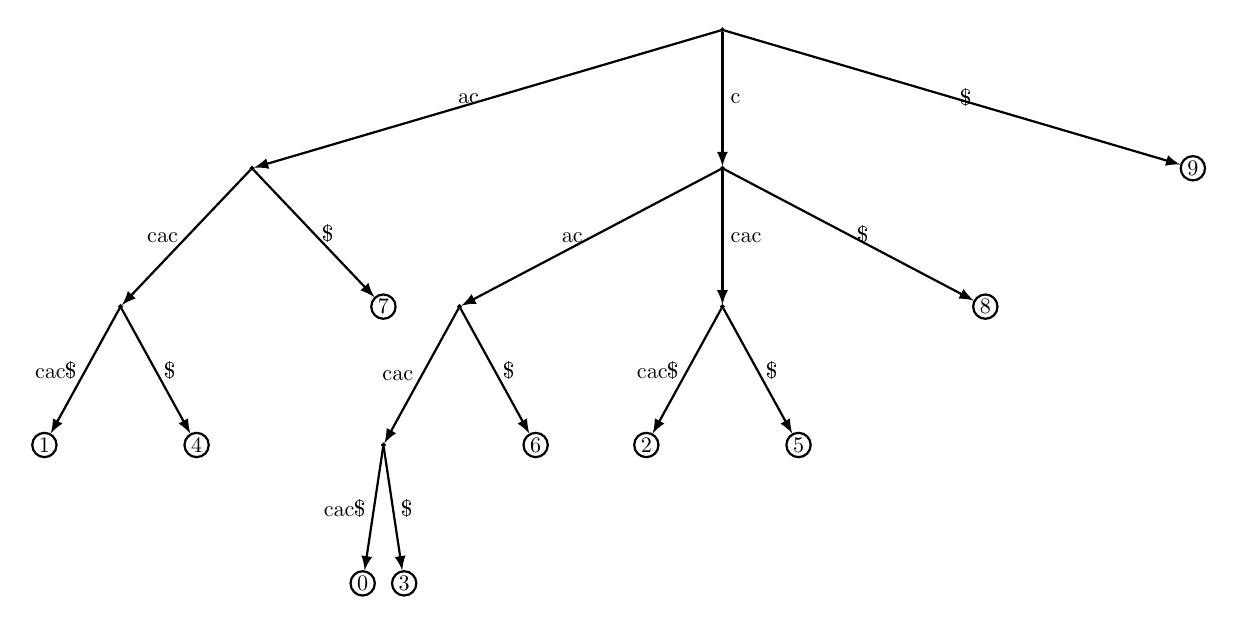
\begin{tikzpicture}[
  >=stealth', thick, level distance=50pt,
  level 1/.style={sibling distance=170pt},
  level 2/.style={sibling distance=95pt},
  level 3/.style={sibling distance=55pt},
  level 4/.style={sibling distance=15pt},
  every node/.style={scale=.8},
  edge from parent/.style={draw,-latex},
  root node/.style={circle,draw,inner sep=0pt},
  leaf node/.style={circle,draw,inner sep=1pt},
  inner node/.style={circle,draw,inner sep=0pt}
]
\node[root node] {}
child {
  node[inner node] {}
  child {
    node[inner node] {}
    child {
      node[leaf node] {1}
      edge from parent node[left] {cac\$}
    }
    child {
      node[leaf node] {4}
      edge from parent node[right] {\$}
    }
    edge from parent node[left] {cac}
  }
  child {
    node[leaf node] {7}
    edge from parent node[right] {\$}
  }
  edge from parent node[left] {ac}
}
child {
  node[inner node] {}
  child {
    node[inner node] {}
    child {
      node[inner node] {}
      child {
        node[leaf node] {0}
        edge from parent node[left] {cac\$}
      }
      child {
        node[leaf node] {3}
        edge from parent node[right] {\$}
      }
      edge from parent node[left] {cac}
    }
    child {
      node[leaf node] {6}
      edge from parent node[right] {\$}
    }
    edge from parent node[left] {ac}
  }
  child {
    node[inner node] {}
    child {
      node[leaf node] {2}
      edge from parent node[left] {cac\$}
    }
    child {
      node[leaf node] {5}
      edge from parent node[right] {\$}
    }
    edge from parent node[right] {cac}
  }
  child {
    node[leaf node] {8}
    edge from parent node[right] {\$}
  }
  edge from parent node[right] {c}
}
child {
  node[leaf node] {9}
  edge from parent node[right] {\$}
}
;
\end{tikzpicture}
\end{center}
\end{document}
